\documentclass[
	%a4paper, % Use A4 paper size
	letterpaper, % Use US letter paper size
]{jdf}
\usepackage{graphicx}
\usepackage{biblatex, float}
\addbibresource{references.bib}


\author{Ali El-Khatib}
\email{aelkhatib6@gatech.edu}
\title{Homework 1}

\begin{document}
\maketitle
\section{Question 1}

\section{Question 2}
\subsection{General Data Protection Regulation \& You}
The General Data Protection Regulation (GDPR) --adopted on April 27, 2016-- is a regulation regarding the protection of personal data and privacy. In effect, it allows users within Europe to have increased control of all personal data (e.g., website cookies, email addresses, phone number). This means that users control the activation of cookies and trackers--methods which collect personal data--on websites they visit. In addition to data control, it enforces a number of other rights for users:
\begin{itemize}
	\item Right to be Forgotten; ability to have data deleted upon request
	\item Right to be notified of data leaks related to their personal data
	\item Right to have data provided in standardized formats (e.g., .csv, .xlsx)
	\item Right to refuse an their data being used in certain processes
\end{itemize}


The GDPR applies in both European Union (EU) member states and the European Economic Area (EEA), both of which are illustrated in Figure~\ref{fig:europe-groups}. 
\begin{figure}[H]
	\centering
	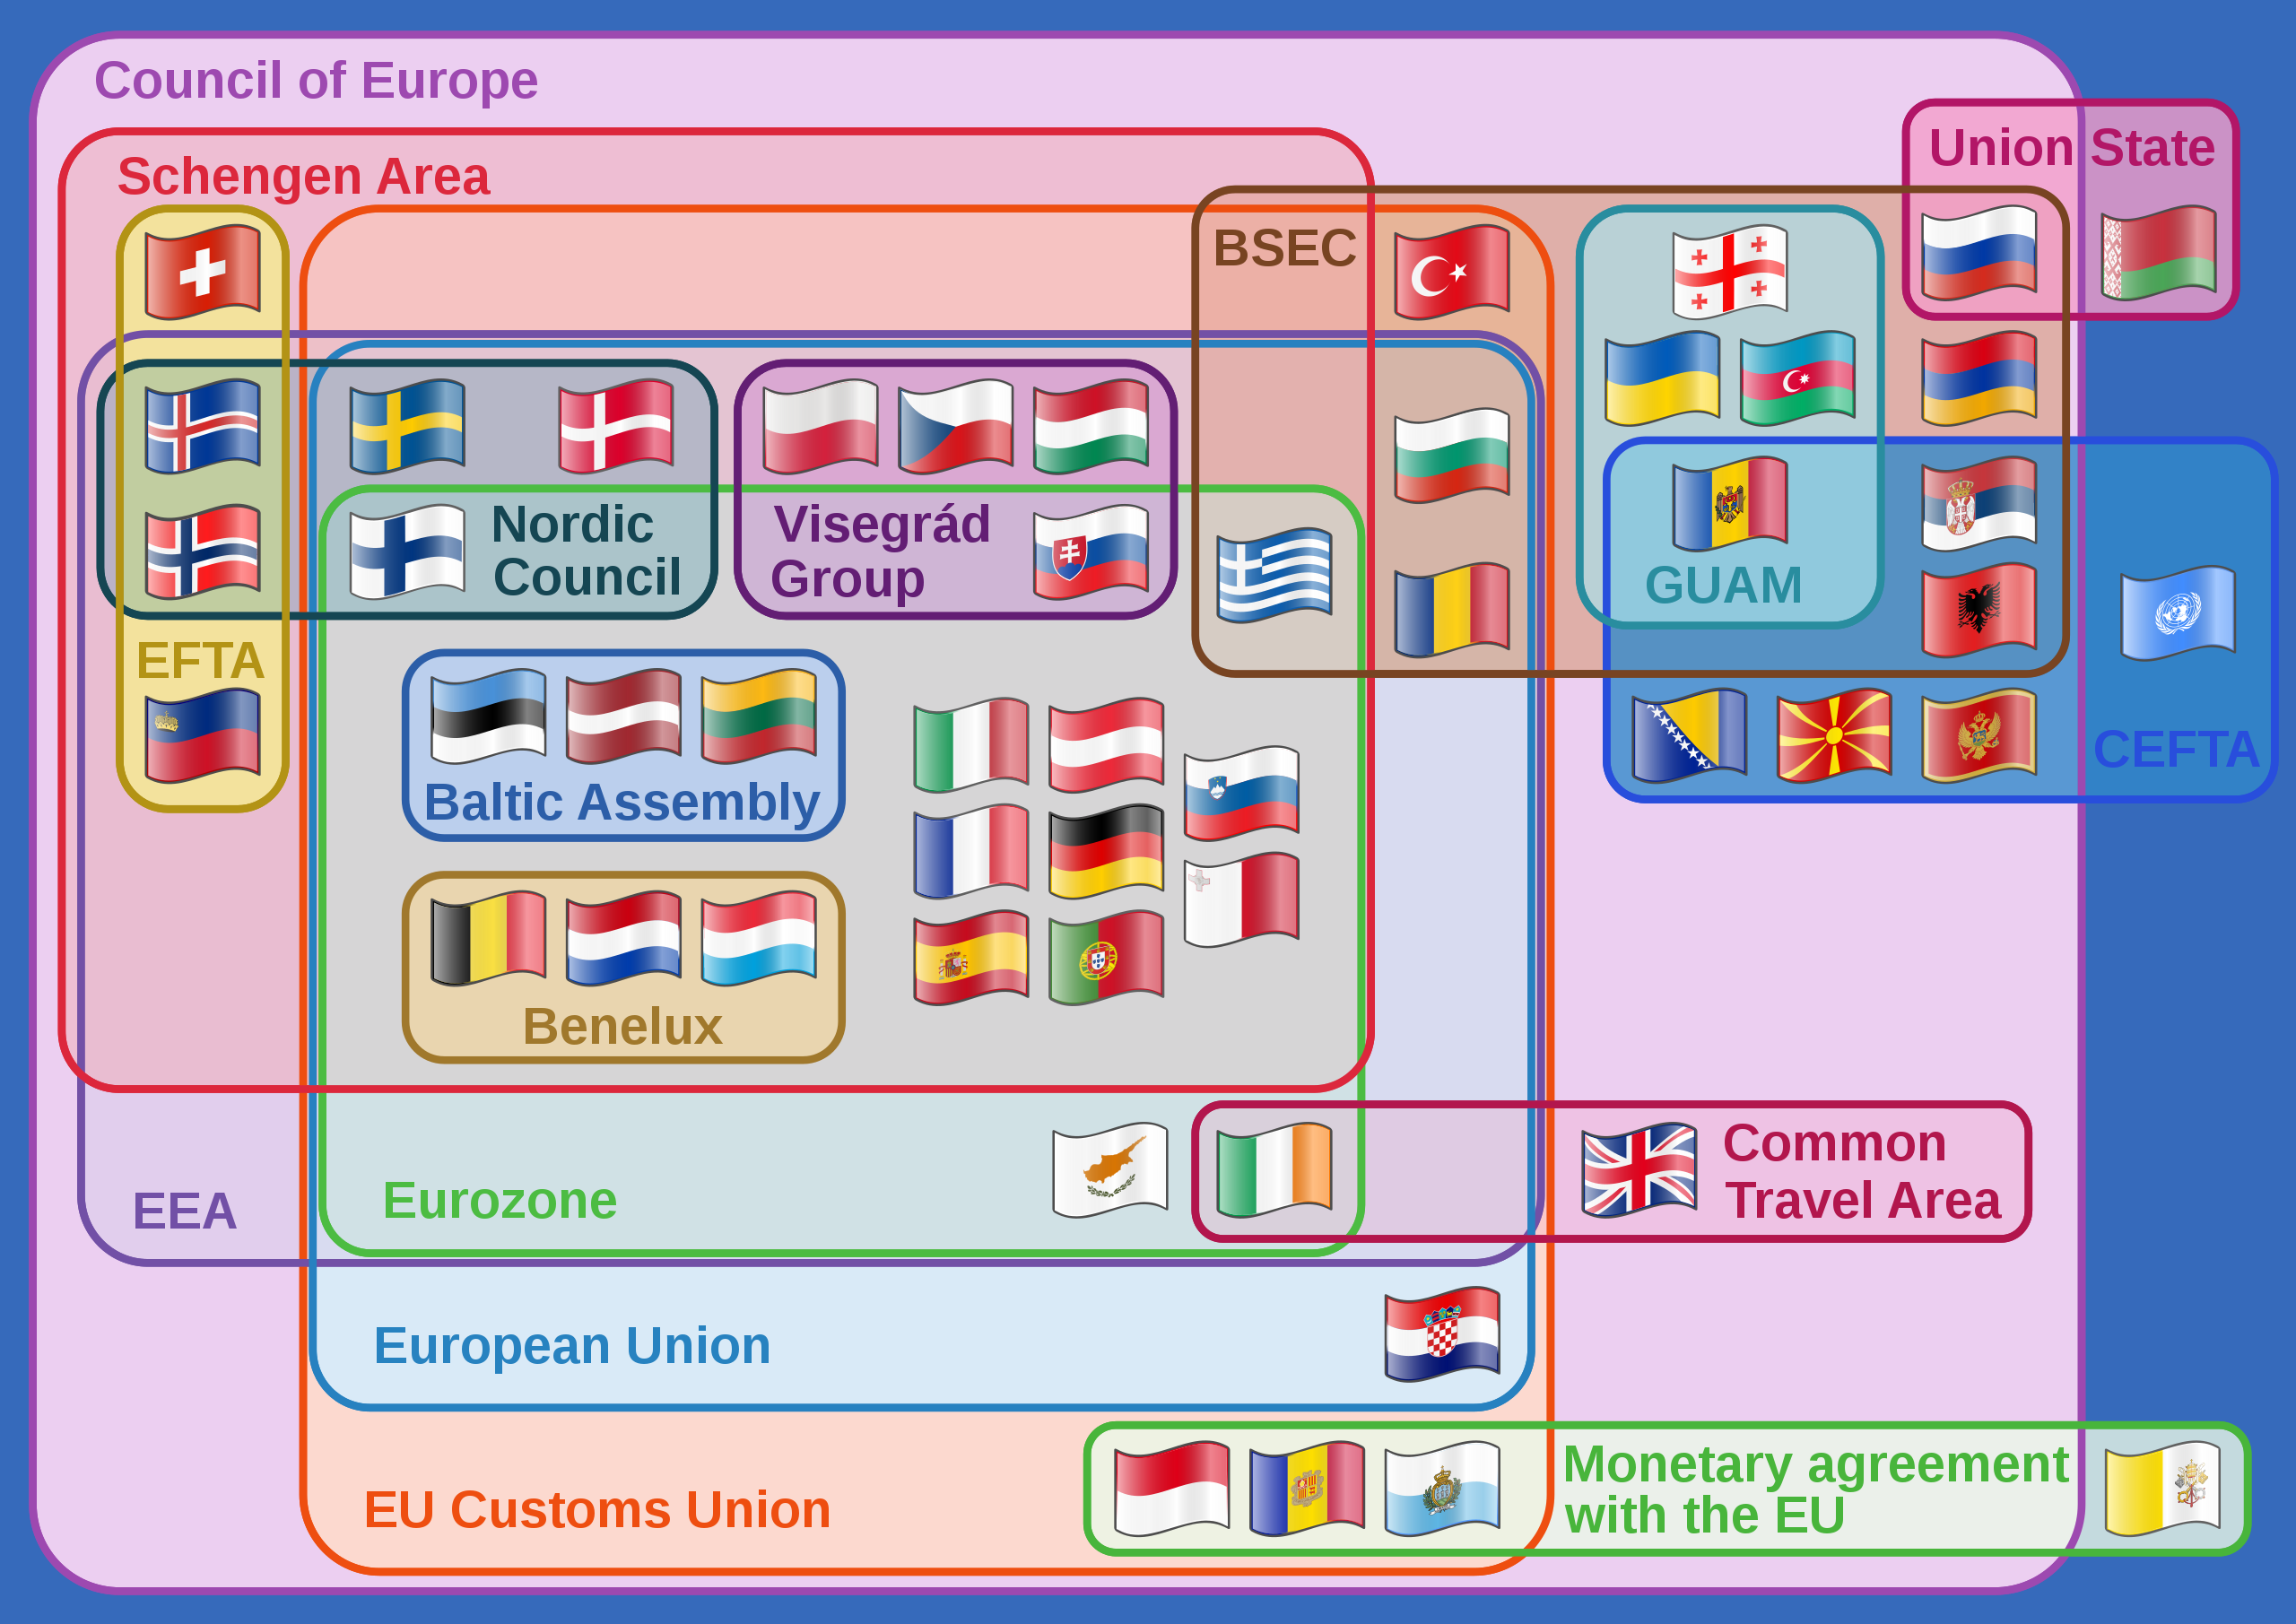
\includegraphics[width=0.7\linewidth]{../figures/europe-groups}
	\caption{Euler Diagram illustrating the various multinational European organizations and agreements. European Union is shown in light blue; EEA is in purple. Source: \href{https://en.wikipedia.org/wiki/File:Supranational_European_Bodies-en.svg}{Wikipedia}
	}
	\label{fig:europe-groups}
\end{figure}

An easily accessible example of the impact of GDPR is Google's Ad personalization, which provides a major revenue source for many websites as well as Google itself. As a result of the GDPR, Google now allows individuals to view the data that is being used to target ads specifically to them. At this moment, anyone with a Google account can go to \href{https://adssettings.google.com/}{Google Ad Settings} and view the process behind Google's ad personalization, shown in \ref{fig:google-ads}. Additionally, it allows the selective removal of an individual's personal info as well as toggling off Ad personalization.

\begin{figure}
	\centering
	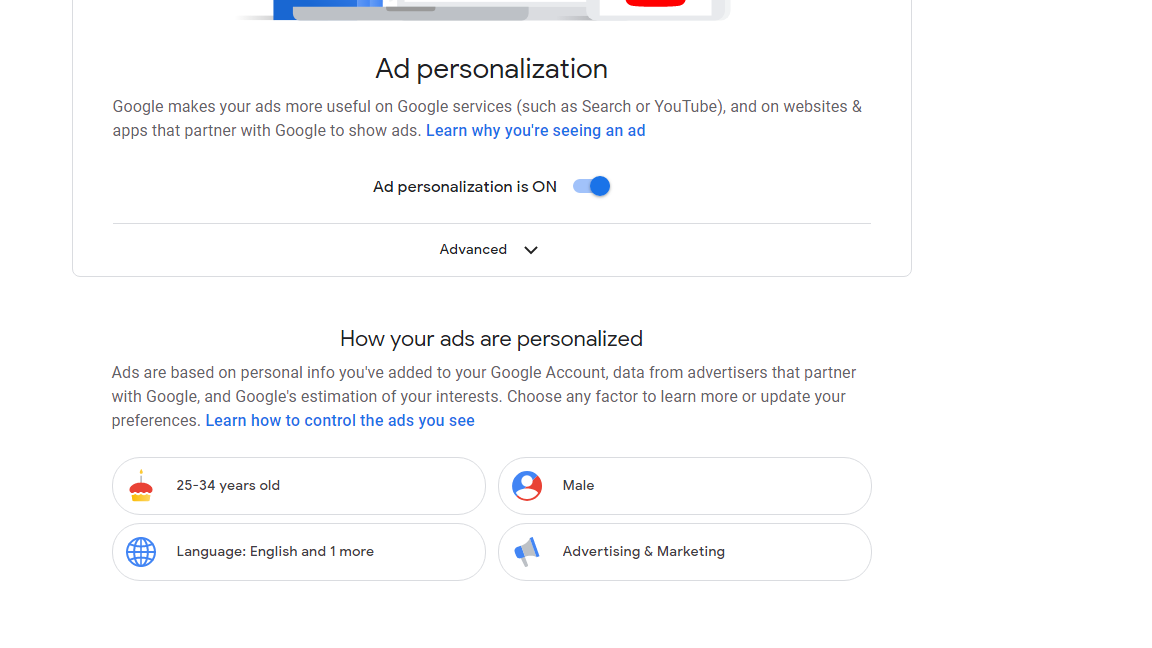
\includegraphics[width=0.7\linewidth]{../figures/google-ads}
	\caption{Example of data Google uses to target ads towards myself (the author)}
	\label{fig:google-ads}
\end{figure}



\end{document}